\documentclass[12pt,a4paper]{report}
\usepackage[T2A]{fontenc}
\usepackage[utf8]{inputenc}
\usepackage[russian]{babel}
\usepackage{graphicx, setspace, hyperref}

\usepackage[
top = 1.25cm, 
bottom = 2.0cm]{geometry}

\begin{document}
\begin{titlepage} 
	\centering
    % HEADER
	{
        \scshape
        Федеральное государственное автономное образовательное учреждение высшего образования
        \par
        \textbf{«Научно-образовательная корпорация ИТМО»}
        \par
        \vspace*{1cm}
        Факультет Программной Инженерии и Компьютерной Техники
        \par
    }
    % LOGO
    \vspace*{0.6cm}
    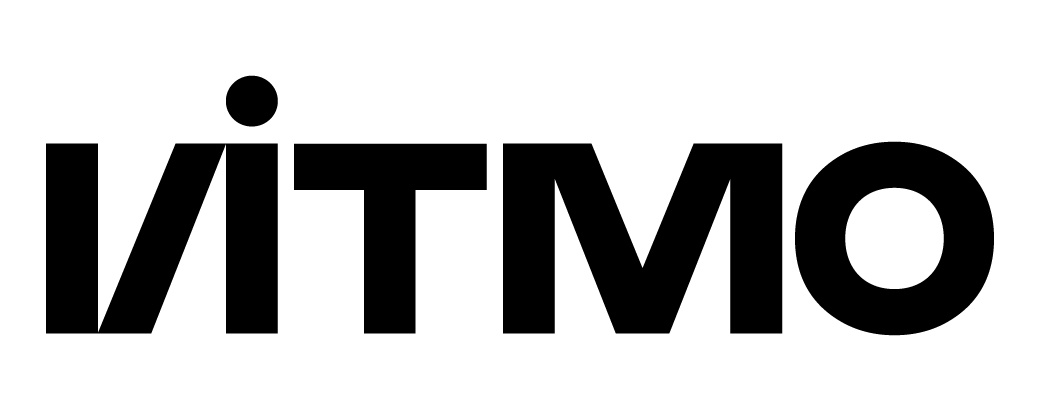
\includegraphics[width=\textwidth]{logo.png}
    % LAB INFO
    {
        \Large
        \textbf{Лабораторная работа по вычислительной математике №1}
        \par
        \normalsize
        \vspace*{0.75cm}
        \textbf{Вариант 13}
        \par
    }
    \vfill
    % СREDITS
    \hfill\begin{minipage}{\dimexpr\textwidth-7.8cm}
        \textbf{Выполнил:}\par
        Степанов Арсений Алексеевич\par
        \vspace*{0.15cm}
        \textbf{Группа:}\par
        P3209\par
        \vspace*{0.15cm}
        \textbf{Преподаватель:}\par
        Наумова Надежда Александровна\par
    \end{minipage}
    \vfill
    Санкт-Петербург, \the\year{}г.
\end{titlepage}  
\section*{Цели}
Разработать консольное приложение находящее решение системы линейных алгебраических уравнений методом простых итераций. Выводить количество итераций, ошибку и промежуточные результаты.
\section*{Методы и расчётные формулы}
Для нахождения решения СЛАУ используется метод простых итераций, исходная система задаётся следующим образом:
$$AX=B$$
На вход подаётся допустимая погрешность вычислений $\delta$ и расширенная матрица задающая СЛАУ $A|B$. Вначале находится нулевое приближение, по следующей формуле:
$$X^{(0)}_i=(\frac{b_i}{A_{ii}})_{N}$$
Следующие приближения находится по следующей формуле:
$$X^{(k+1)}_i=\frac{1}{a_{ii}}(b_i -\sum_{i\not=j}X^{(k)}_ia_{ij}) $$
Отклонения находятся по следующей формуле:
$$D_i=\frac{ |X^{(k+1)} - X^{(k)}| }{|X^{(k+1)}|}$$
Итерации продолжаются до тех пор, пока не выполнится условие:
$$D_i \leq \delta$$
\section*{Блок-схема программы}
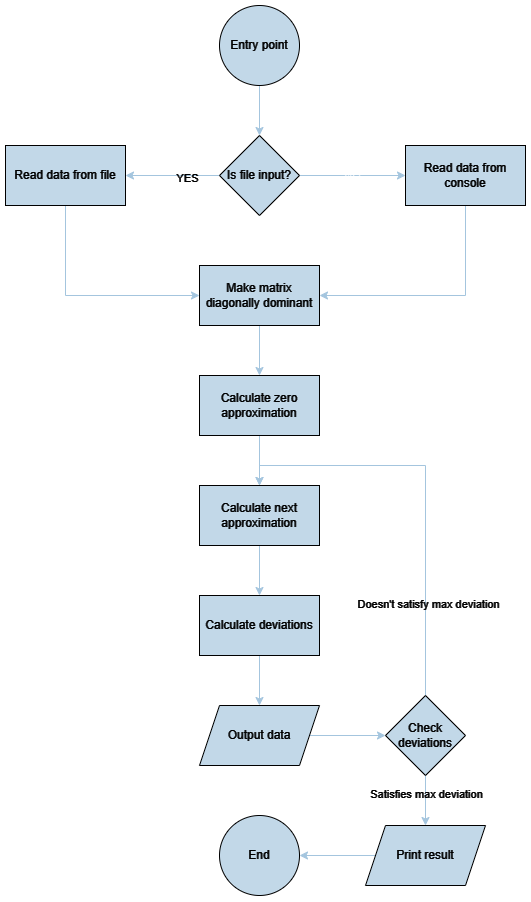
\includegraphics[width=\textwidth]{schema.png}
\section*{Итоговый результат}
Ссылка на репозиторий с кодом \href{https://github.com/Armemius/ComputationalMathLab1}{GitHub}
\section*{Выводы}
Я познакомился с методами решения СЛАУ с использованием компьютерной мощностей и реализовал на практике программу для нахождения решения СЛАУ методом простых итераций
\end{document}